\documentclass{article}
\usepackage[margin=.9in]{geometry}
\usepackage{xcolor}
\usepackage{amsmath}
\usepackage{amssymb}
\usepackage{float}
\usepackage{listings}
\usepackage{booktabs}
\lstset{
  basicstyle=\small\ttfamily,
  breaklines=true,
  frame=single,
  language=Verilog,
  numberstyle=\tiny,
  showstringspaces=false
}
\setlength{\parindent}{0pt}
\setlength{\parskip}{\baselineskip}
\definecolor{mycolor}{rgb}{0.1, 0.1, 0.5}
\title{\textbf{{\huge Voltage Controlled Oscillator Design}}}
\author{Christopher Hunt}
\date{}
\usepackage{graphicx} 
\usepackage{fancyhdr}

\begin{document}
\pagestyle{fancy}
\fancyhf{}
\rfoot{ENGR 203}
\lfoot{Christopher Hunt}
\lhead{VCO Design}
\rhead{\thepage}
\maketitle
\section*{\textcolor{mycolor}{Objective}}
The aim of this lab is to design and analyze a simple sawtooth oscillator based on an inverting Schmitt trigger circuit designed by Moritz Klein. The oscillator's frequency is controlled by a voltage input, which modulates the behavior of an NPN transistor. We will investigate the signals that control the NPN transistor and study its response characteristics. The project will involve building the oscillator circuit, implementing signal analysis techniques, and exploring the effects of different control voltages on the oscillator's output waveform.

To accomplish the objectives of this lab project, we will first construct the sawtooth oscillator circuit using an inverting Schmitt trigger and NPN transistor. We will then examine the behavior of the NPN transistor by studying the signals that control its openness. Additionally, operational amplifiers and AC coupling will be used to eliminate DC offset and enhance the quality of the output waveform.

Through this project, we will gain insights into voltage-controlled oscillators, NPN transistor behavior, and the impact of control signals on the oscillator's output.
\vspace{5mm}
\hrule

\section*{\textcolor{mycolor}{Equipment}}
\begin{itemize}
  \item Siglent SDS 1202X-E Serial: SDS1EDEQ6R7384
  \item HP 6236B Triple Output Power Supply Serial: 15175
  \item AstroAI DM6000AR Multimeter
  \item Korg SQ-1 Serial: 048860
\end{itemize}
\vspace{5mm}
\hrule

\section*{\textcolor{mycolor}{Design}}
A Voltage Controlled Oscillator (VCO) is an electronic circuit that utilizes an input voltage to regulate and modify the frequency of the generated oscillating waveform. In this lab, the VCO design centers around an inverting Schmitt Trigger, which incorporates hysteresis with two distinct trigger points: a higher threshold voltage ($V_{High}$) and a lower threshold voltage ($V_{Low}$).

In this specific design, an inverting Schmitt Trigger is carefully selected to achieve the desired functionality. When the circuit is powered, the Schmitt Trigger initially produces a high signal. Once the input voltage surpasses the $V_{High}$ threshold, the output switches to a low signal. Conversely, when the input voltage drops below the $V_{Low}$ threshold, the output switches back to a high signal. This behavior is achieved by employing a diode to feed the trigger's output back to its input.

To introduce the voltage-controlled behavior of the oscillator, a capacitor is connected to the same input node as the Schmitt Trigger. Upon powering the circuit, the capacitor starts to charge. As soon as the voltage on the capacitor reaches the $V_{High}$ threshold, the Schmitt Trigger turns off, causing the capacitor to discharge. This discharge process extends the duration during which the input voltage remains above the $V_{Low}$ threshold.

The rate at which the capacitor discharges can be precisely controlled by adjusting the resistance between the input node and ground. Placing a potentiometer at this point enables manual adjustment of the oscillator's frequency. Alternatively, this adjustment can be automated using transistors. By replacing the potentiometer with an NPN transistor between the input and ground, the amount of current passing from the input node to ground can be modulated by varying the voltage at the transistor's base.

For this specific design, a combination of NPN and PNP transistors is employed, with the PNP transistor configured as an emitter follower. This arrangement effectively addresses potential temperature effects that might challenge a single transistor in maintaining a constant current, potentially impacting the frequency of the sawtooth wave. The NPN and PNP transistors essentially operate in an inverse manner with respect to temperature. As the temperature rises, the NPN transistor opens up, allowing more current to flow. Conversely, the PNP transistor starts to restrict current flow, raising the voltage at the base of the NPN transistor. This process counteracts the temperature's influence, resulting in more stable capacitor drainage and, consequently, a more consistent output frequency.

To facilitate voltage control, the base of the PNP transistor serves as the control point. A simulated potentiometer, achieved by a voltage divider between $V_{pos}$ and $V_{neg}$, allows for setting the lowest frequency when the control voltage is at zero. The external voltage signals applied at $VC$ can then modify the frequency by modulating the voltage applied to the base, providing the VCO with versatile control options.

Subsequently, the generated sawtooth wave is directed to the positive terminal of an amplifier circuit. This circuit plays a crucial role in decoupling the generator from the output, removing any DC offset using AC coupling, and amplifying the output to an appropriate voltage range for subsequent signal processing.

By implementing these components and configurations, the VCO design achieves precise voltage-controlled frequency modulation and incorporates measures to compensate for temperature effects, ensuring stable performance and facilitating signal processing in further stages.


\begin{figure}[H]
  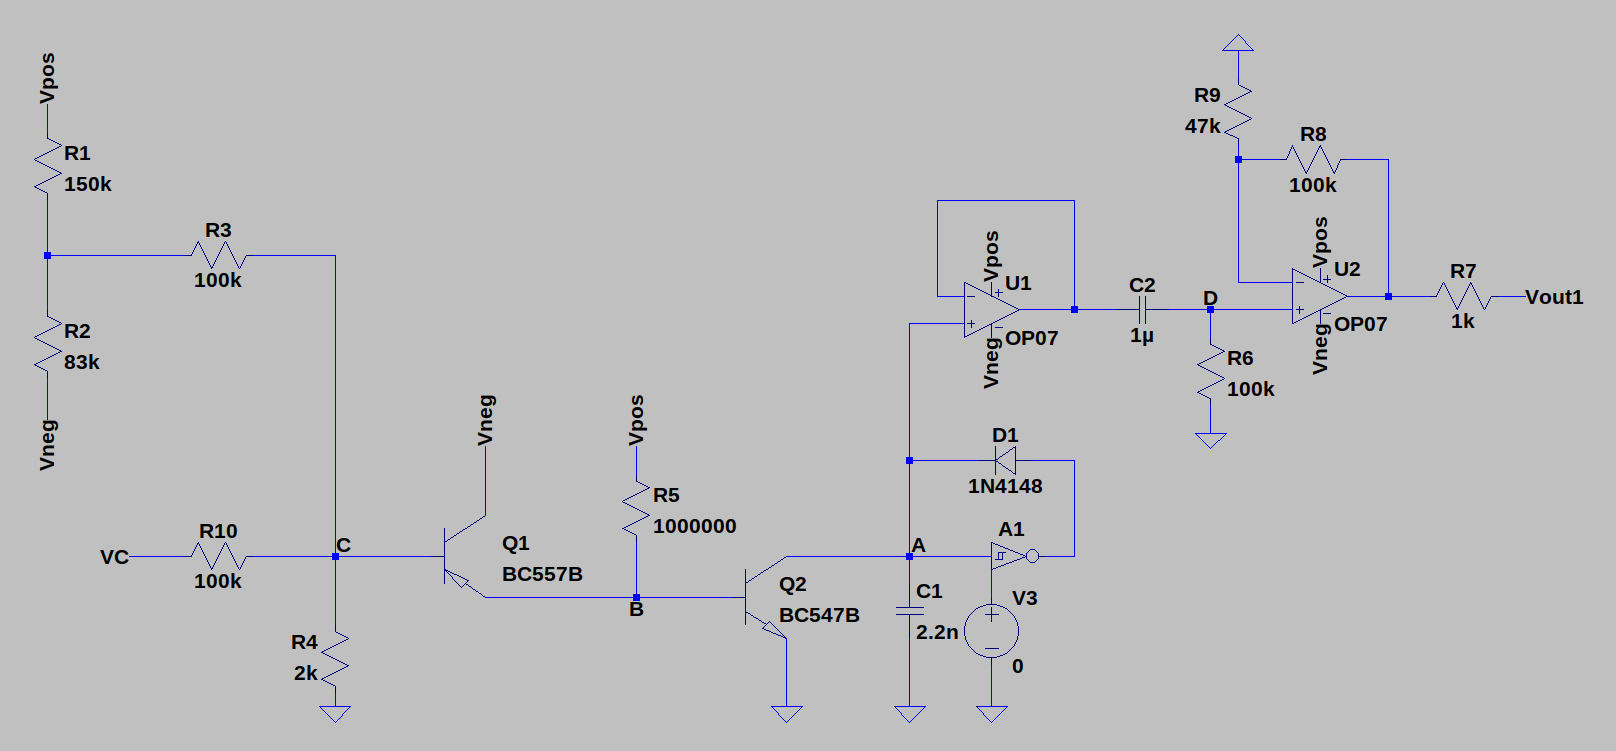
\includegraphics[width=1\linewidth]{png/vco_schem.png}
  \caption{VCO Schematic}
\end{figure}


\section*{\textcolor{mycolor}{Simulation}}
We will focus on analyzing five primary nodes in this circuit. Node A serves as the starting point for the sawtooth oscillator. Nodes B and C play a crucial role in regulating the flow of charge, allowing it to either pass to ground from C1 or reducing its flow. Node D represents the AC coupling junction, responsible for eliminating the DC offset from the original sawtooth signal. Lastly, we have $V_{out1}$, which denotes the final output of the Voltage-Controlled Oscillator (VCO).

To conduct the simulation, we will use LTSpice. The primary objective of the simulation is to observe the circuit's complete range when the potentiometer is fully open or closed. This will enable us to determine the full frequency range of the sawtooth oscillator. Subsequently, we will test the VC input, expecting the control voltage at VC to vary between 0 and 5 volts. Our goal is for the VCO to increase in frequency on a 1-volt-per-octave scale.

Once we have thoroughly analyzed the control side of the circuit, our next step will involve examining the output AC coupling and amplification.

To test the high-frequency range, we will begin with these conditions on the control side of the circuit: the voltage at VC will be zero, $V_{pos} = +9 V$, and $V_{neg} = -9 V$, $R_1 = 100k \Omega$, and $R_2 = 133k \Omega$. Voltage levels are taken at nodes A, B, and C.

\begin{table}[H]
  \centering
  \begin{tabular}{ll}
    \toprule
    Parameter & Value \\
    \midrule
    $R_1$ & 100k \\
    $R_2$ & 133k \\
    NPN Base Voltage ($V_B$) & 0.521V \\
    PNP Base Voltage ($V_C$) & 0.00201V \\
    Oscillator Frequency & 5,334Hz \\
    \bottomrule
  \end{tabular}
  \caption{High-Frequency Inputs and Oscillator Response}
\end{table}
\vspace{-1.5cm}
\begin{figure}[H]
  \centering
  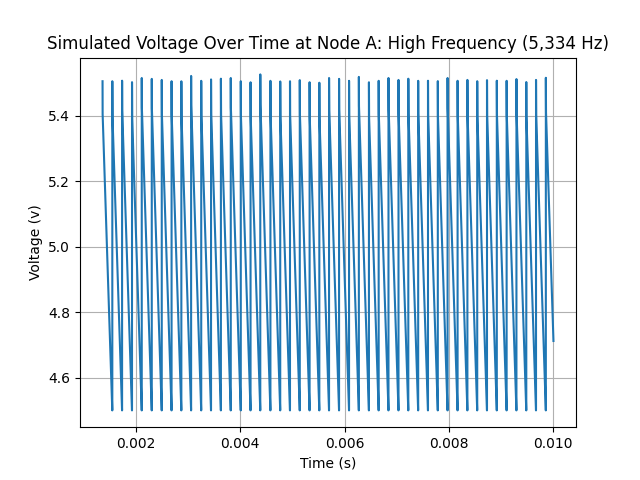
\includegraphics[width=.7\linewidth]{png/Figure_1.png}
  \caption{High-Frequency Simulation | Voltage at Node A}
\end{figure}

To test the low-frequency range, we will begin with these conditions on the control side of the circuit: the voltage at VC will be zero, $V_{pos} = +9 V$, and $V_{neg} = -9 V$, $R_1 = 200k \Omega$, and $R_2 = 33k \Omega$. Voltage levels are taken at nodes A, B, and C.

\begin{table}[H]
  \centering
  \begin{tabular}{ll}
    \toprule
    Parameter & Value \\
    \midrule
    $R_1$ & 200k $\Omega$ \\
    $R_2$ & 33k $\Omega$ \\
    NPN Base Voltage ($V_B$) & 0.370 V \\
    PNP Base Voltage ($V_C$) & -0.1302 V \\
    Oscillator Frequency & 18 Hz \\
    \bottomrule
  \end{tabular}
  \caption{Low-Frequency Inputs and Oscillator Response}
\end{table}
\vspace{-1.5cm}
\begin{figure}[H]
  \centering
  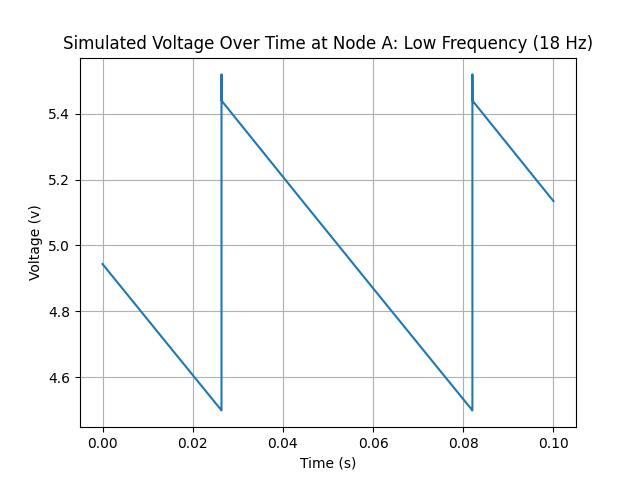
\includegraphics[width=.7\linewidth]{png/Figure_2.png}
  \caption{Low-Frequency Simulation | Voltage at Node A}
\end{figure}


The frequency range of the Oscillator is between 18 Hz and 5,334 Hz. By varying the voltage divider that is created between $V_{pos}$ and $V_{neg}$, we are able to control the speed with which the drain capacitor, $C_1$, discharges. Next, we will simulate the effects of the $VC$ input. Simulations will be done for inputs of 0 to 5 volts at 1-volt increments. The base frequency will be kept at the Oscillator's low value.

\begin{table}[H]
  \centering
  \begin{tabular}{cc}
    \toprule
    \textbf{CV Input Voltage (V)} & \textbf{Frequency (Hz)} \\
    \midrule
    0 & 18 \\
    1 & 36.23 \\
    2 & 74.41 \\
    3 & 154.2 \\
    4 & 321.0 \\
    5 & 669.4 \\
    \bottomrule
  \end{tabular}
  \caption{CV Input Voltage and Frequency}
\end{table}

\begin{figure}[H]
  \centering
  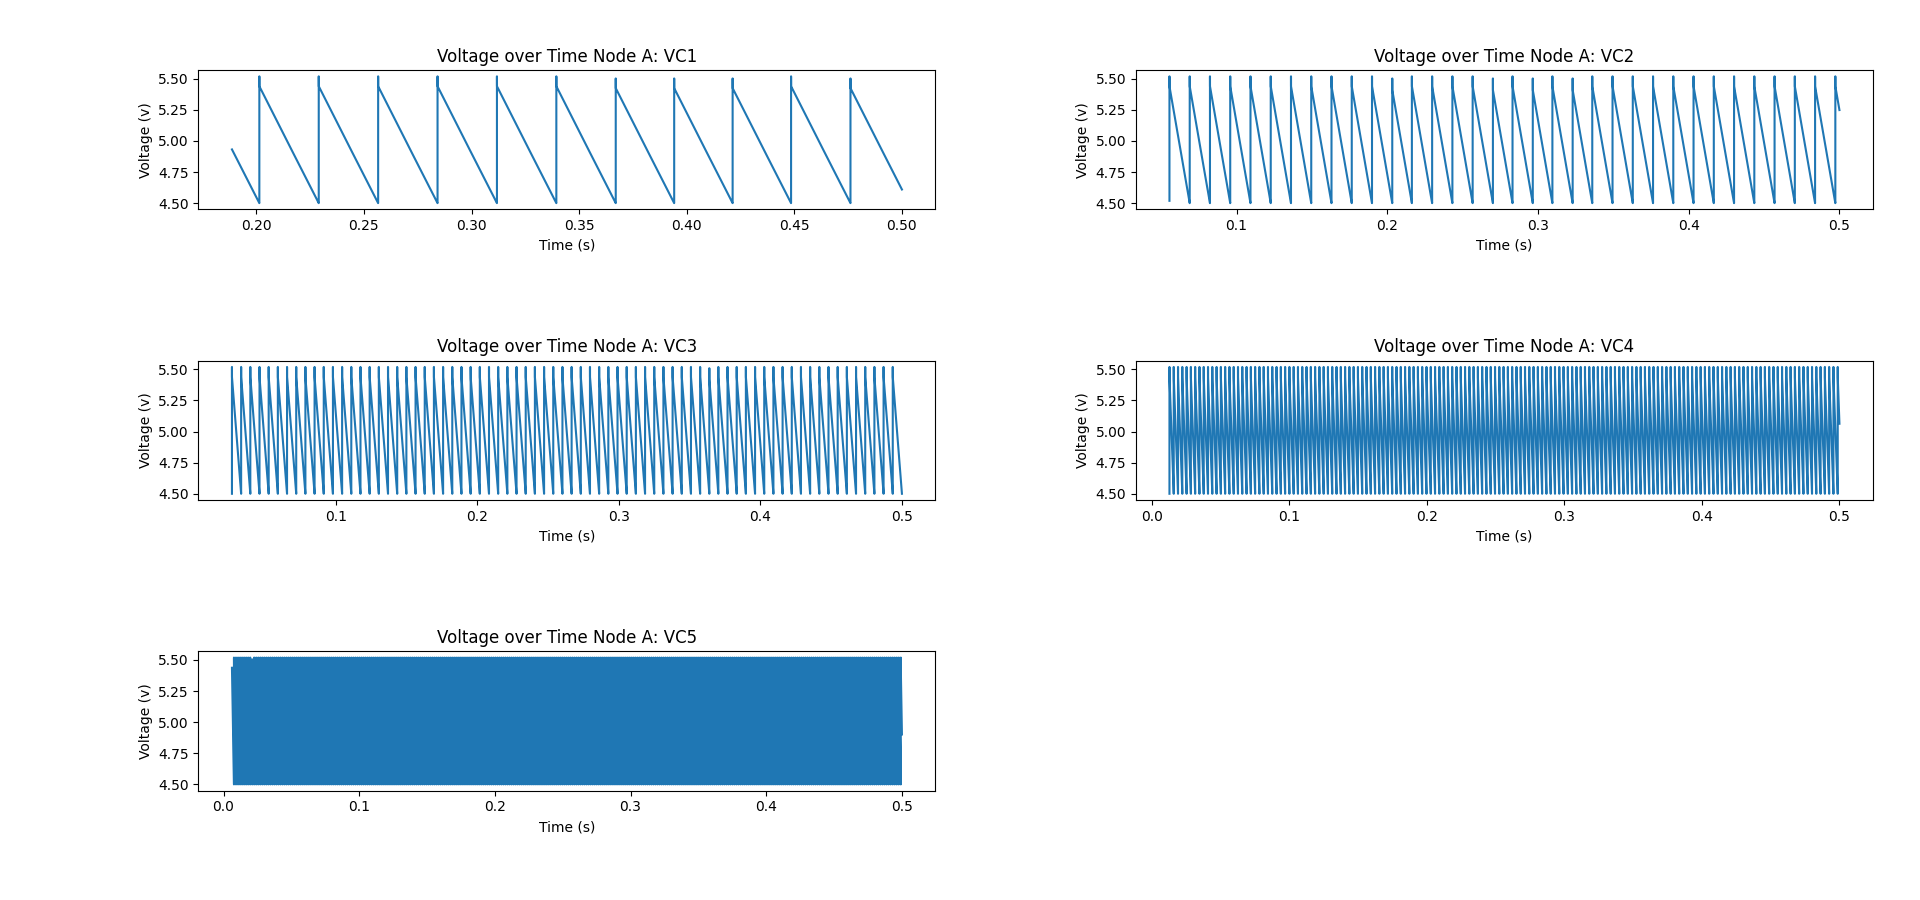
\includegraphics[width=.7\linewidth]{png/Figure_3.png}
  \caption{Control Voltage Simulations: 0 - 5 volts}
\end{figure}

When the CV input is increased by 1-volt increments from 0 to 5 volts, the output frequency doubles correspondingly. This exponential frequency increase aligns with the desired mapping of frequency to the 1 octave per volt standard commonly used for voltage-controlled oscillators.

Next we will investigate Node D and the final output $V_{out1}$ (Figures 5 and 6). At Node D we see the signal is now centered around 0 volts with a peak to peak voltage of .91 volts.

\begin{figure}[H]
  \centering
  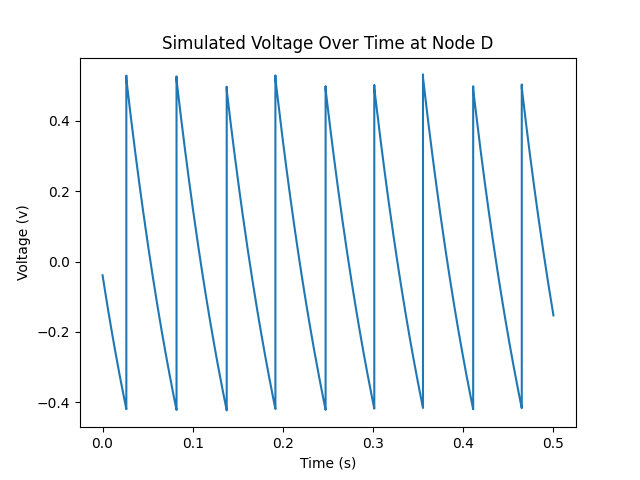
\includegraphics[width=.7\linewidth]{png/nodeD.png}
  \caption{Node D: AC Coupling to Remove DC offset}
\end{figure}

After the DC offset has been removed, the signal is again amplified and the final output is measured to be 2.83 volts peak to peak.

\begin{figure}[H]
  \centering
  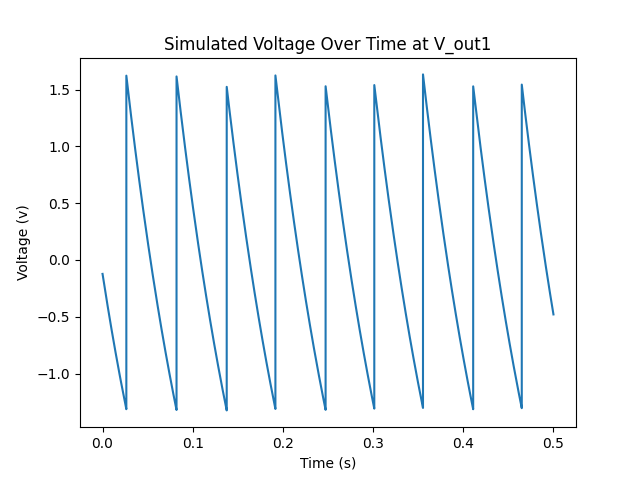
\includegraphics[width=.7\linewidth]{png/Vout1.png}
  \caption{$V_{out1}$: Final output of VCO}
\end{figure}

\vspace{5mm}
\hrule
  
\section*{\textcolor{mycolor}{Implementation}}
Implementation is next. The circuit was built out on a breadboard (Figure 5). In this design, a potentiometer was used for coarse tuning, and a 1k $\Omega$ trim pot and 1k $\Omega$ in series were used for $R_4$ to aid in attaining the desired voltage at the base of the PNP transistor.

\begin{figure}[H]
  \centering
  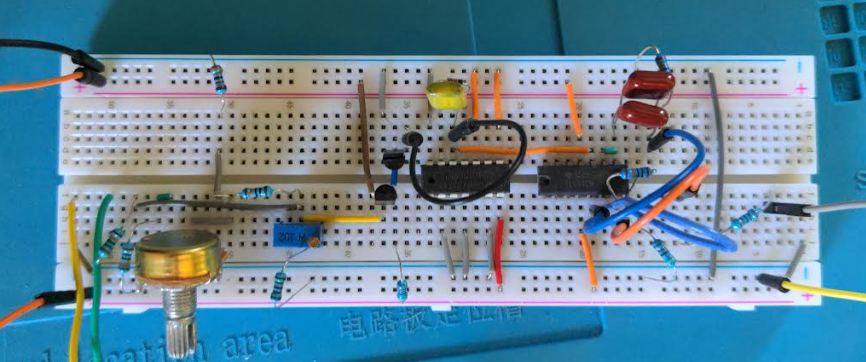
\includegraphics[width=.89\linewidth]{png/vco_breadboard.png}
  \caption{Breadboarded VCO Circuit}
\end{figure}

First, we will simulate the maximum frequency of the oscillator (Figure 6). With this circuit configuration, the maximum frequency attained is 4854 Hz.

\begin{figure}[H]
  \centering
  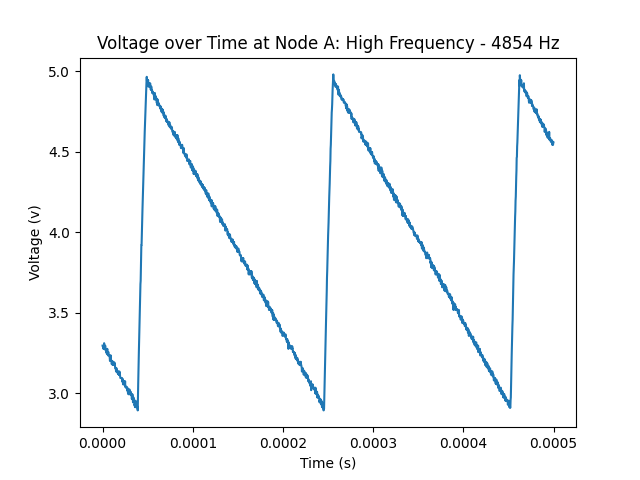
\includegraphics[width=.7\linewidth]{png/Figure_5.png}
  \caption{High Frequency | Voltage at Node A}
\end{figure}

Next, we will simulate the minimum frequency of the oscillator (Figure 7). With this circuit configuration, the minimum frequency attained is 18.5 Hz.

\begin{figure}[H]
  \centering
  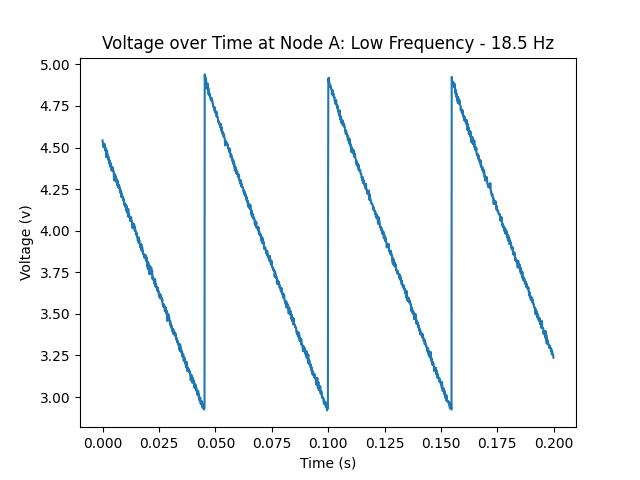
\includegraphics[width=.7\linewidth]{png/Figure_4.png}
  \caption{Low Frequency | Voltage at Node A}
\end{figure}

To test the voltage-controlled behavior of the oscillator, testing was performed by varying control voltages (CV) ranging from 0 to 5 volts in 1-volt increments. The corresponding PNP transistor voltage, NPN transistor voltage, and oscillator frequency were recorded for each control voltage (Table 4).

\begin{table}[H]
  \centering
  \begin{tabular}{cccccc}
    \toprule
    \textbf{CV} & \textbf{PNP Voltage} & \textbf{NPN Voltage} & \textbf{Frequency} \\
    \midrule
    0 & -0.129 V & 0.461 V & 18.5 Hz \\
    1.01  & -0.0979 V & 0.492 V  & 53.2 Hz\\
    2.002 & -0.0701 V & 0.519 V  & 148.7 Hz\\
    3.046  & -0.0399 V & 0.549 V & 467.1 Hz\\
    4.01 & -0.0143 V & 0.56 V & 1255 Hz\\
    5.01 & 0.0134 V & 0.602 V & 3610 Hz\\
  \end{tabular}
  \caption{CV Input Voltage and Corresponding PNP and NPN Voltage and Output Frequency}
\end{table}

\begin{figure}[H]
  \centering
  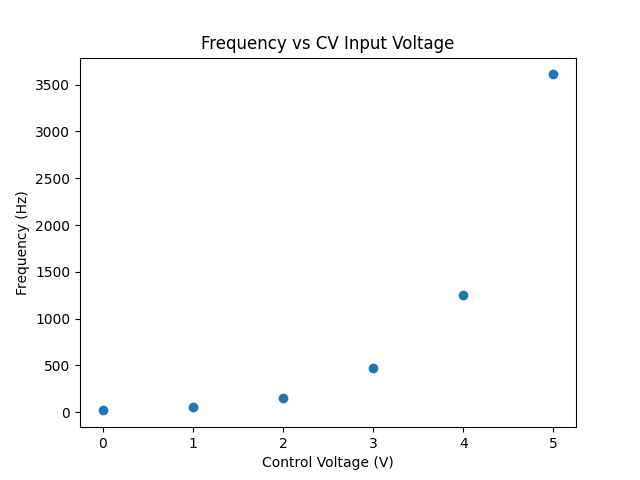
\includegraphics[width=.7\linewidth]{png/Figure_6.png}
  \caption{Control Voltage Implementation: 0 - 5 volts}
\end{figure}

\vspace{5mm}
\hrule
  
\section*{\textcolor{mycolor}{Conclusion}}

The Voltage Controlled Oscillator (VCO) design proved to be successful in achieving its objective of creating a functional and versatile oscillator circuit. By comparing the simulated values with the implemented values, we can assess the performance and identify any discrepancies.

During simulation, the VCO circuit exhibited the expected behavior, with the frequency range aligning closely with the simulated values. However, upon implementation on a breadboard, there were slight deviations between the simulated and implemented values.

Specifically, in the high-frequency range, the implemented circuit demonstrated a maximum frequency of 4,854 Hz, slightly lower than the simulated value of 5,334 Hz. This discrepancy may be attributed to the limitations and non-idealities of the physical components used in the breadboard implementation, such as variations in component tolerances and parasitic effects.

In the low-frequency range, the implemented circuit achieved a minimum frequency of 18.5 Hz, which closely matched the simulated value. This suggests that the circuit design was effective in producing the desired low-frequency output.

When varying the control voltage (CV) from 0 to 5 volts in 1-volt increments, the implemented circuit exhibited frequency responses that closely resembled the simulated results. However, minor variations between the simulated and implemented values were observed, possibly due to factors such as component tolerances and non-linearities of the transistors.

Despite these discrepancies, the implemented VCO design still achieved its main objectives of generating a voltage-controlled sawtooth waveform and providing frequency modulation based on the control voltage. The circuit demonstrated the anticipated exponential increase in frequency with increasing control voltage, indicating the successful incorporation of voltage control.
\vspace{5mm}
\hrule

\end{document}
